\documentclass[tikz,border=0pt]{standalone}

\usepackage{fontspec}
\defaultfontfeatures{Ligatures=TeX}
\setmainfont{Arial}
\setsansfont{Arial}
\renewcommand{\familydefault}{\sfdefault}

\usepackage{amsmath,amssymb,bm}
\usepackage[italic]{mathastext}
\usepackage{tikz}
\usetikzlibrary{arrows.meta,calc,fit,positioning,shapes.geometric}

\definecolor{FigBlue}{HTML}{2C78D0}
\definecolor{FigGreen}{HTML}{2E8B57}
\definecolor{FigOrange}{HTML}{C96A00}
\definecolor{FigRed}{HTML}{C74A44}
\definecolor{FigDark}{HTML}{202020}
\definecolor{FigGrid}{HTML}{D9D9D9}
\definecolor{FigLight}{HTML}{F4F4F4}
\definecolor{FigActorFill}{HTML}{F6F9FC}
\definecolor{FigFormulaFill}{HTML}{FCF8F6}

\newcommand{\RThreeTitle}{\fontsize{8.9}{9.8}\selectfont\bfseries}
\newcommand{\RThreeText}{\fontsize{7.35}{8.0}\selectfont}
\newcommand{\RThreeSmall}{\fontsize{6.75}{7.35}\selectfont}
\newcommand{\RThreeTiny}{\fontsize{6.25}{6.9}\selectfont}
\newcommand{\RThreeFormula}{\fontsize{6.85}{7.45}\selectfont}
\newcommand{\RThreeTerminal}{\fontsize{8.1}{8.9}\selectfont\bfseries}

\tikzset{
  r3base/.style={
    draw=FigDark,
    fill=FigLight,
    line width=0.9pt,
    align=center,
    inner sep=2.2pt,
    text=FigDark,
    font=\RThreeText
  },
  flowbox/.style={r3base, rectangle, draw=FigBlue, font=\RThreeTiny},
  stepbox/.style={r3base, rectangle, draw=FigGreen, fill=white},
  neutralbox/.style={r3base, rectangle, draw=FigGrid, fill=white},
  actorbox/.style={r3base, rectangle, draw=FigBlue, fill=FigActorFill},
  targetbox/.style={actorbox, dashed, line width=0.9pt},
  formulabox/.style={r3base, rectangle, draw=FigOrange, fill=FigFormulaFill},
  terminalbox/.style={
    r3base,
    ellipse,
    draw=FigBlue,
    fill=white,
    line width=1.0pt,
    font=\RThreeTerminal
  },
  decisionbox/.style={
    r3base,
    diamond,
    aspect=2.25,
    draw=FigOrange,
    fill=white,
    line width=1.0pt,
    inner sep=0.8pt,
    font=\RThreeTiny
  },
  outercallout/.style={
    draw=FigRed,
    dashed,
    line width=0.9pt,
    rounded corners=1pt,
    fill=none
  },
  mainarrow/.style={
    -{Latex[length=1.55mm,width=0.95mm]},
    draw=FigDark,
    line width=1.0pt,
    shorten >=4.0pt,
    shorten <=2.0pt
  },
  subarrow/.style={
    -{Latex[length=1.45mm,width=0.90mm]},
    draw=FigDark,
    line width=0.85pt,
    shorten >=3.5pt,
    shorten <=2.0pt
  },
  softarrow/.style={
    -{Latex[length=1.45mm,width=0.90mm]},
    draw=FigDark,
    dashed,
    line width=0.85pt,
    shorten >=3.5pt,
    shorten <=2.0pt
  },
  arrowlabel/.style={
    fill=white,
    inner sep=1.0pt,
    text=FigDark,
    font=\RThreeTiny
  }
}


\begin{document}
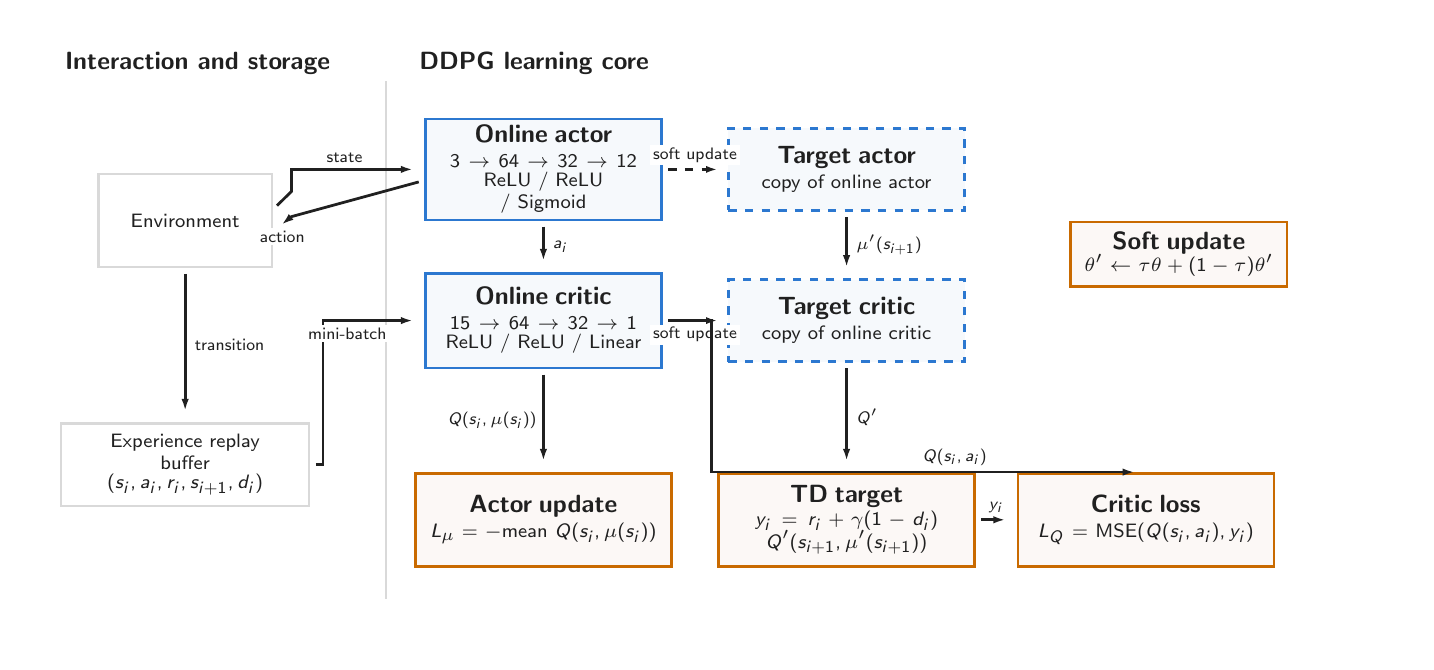
\begin{tikzpicture}[x=1cm,y=1cm]
\path[use as bounding box] (0,0) rectangle (17.5,7.8);

\node[font=\RThreeTitle, text=FigDark, anchor=west] at (0.35,7.35) {Interaction and storage};
\node[font=\RThreeTitle, text=FigDark, anchor=west] at (4.85,7.35) {DDPG learning core};
\draw[FigGrid, line width=0.8pt] (4.55,0.55) -- (4.55,7.12);

\node[neutralbox, minimum width=2.20cm, minimum height=1.18cm, text width=1.82cm] (env) at (2.00,5.35)
  {Environment};
\node[neutralbox, minimum width=3.15cm, minimum height=1.05cm, text width=2.72cm] (replay) at (2.00,2.25)
  {Experience replay\\buffer\\[-1pt]{\RThreeSmall $(s_i,a_i,r_i,s_{i+1},d_i)$}};

\node[actorbox, minimum width=3.00cm, minimum height=1.20cm, text width=2.68cm] (onlineactor) at (6.55,6.00)
  {{\RThreeTitle Online actor}\\[1pt]
  {\RThreeFormula $3\to64\to32\to12$}\\[-1pt]
  {\RThreeSmall ReLU / ReLU / Sigmoid}};
\node[actorbox, minimum width=3.00cm, minimum height=1.20cm, text width=2.68cm] (onlinecritic) at (6.55,4.08)
  {{\RThreeTitle Online critic}\\[1pt]
  {\RThreeFormula $15\to64\to32\to1$}\\[-1pt]
  {\RThreeSmall ReLU / ReLU / Linear}};

\node[targetbox, minimum width=3.00cm, minimum height=1.04cm, text width=2.68cm] (targetactor) at (10.40,6.00)
  {{\RThreeTitle Target actor}\\[1pt]
  {\RThreeSmall copy of online actor}};
\node[targetbox, minimum width=3.00cm, minimum height=1.04cm, text width=2.68cm] (targetcritic) at (10.40,4.08)
  {{\RThreeTitle Target critic}\\[1pt]
  {\RThreeSmall copy of online critic}};

\node[formulabox, minimum width=3.25cm, minimum height=1.18cm, text width=2.93cm] (actorupdate) at (6.55,1.55)
  {{\RThreeTitle Actor update}\\[1pt]
  {\RThreeFormula $L_\mu=-\mathrm{mean}\ Q(s_i,\mu(s_i))$}};
\node[formulabox, minimum width=3.25cm, minimum height=1.18cm, text width=2.93cm] (tdtarget) at (10.40,1.55)
  {{\RThreeTitle TD target}\\[1pt]
  {\RThreeFormula $y_i=r_i+\gamma(1-d_i)$\\[-1pt]
  $Q'(s_{i+1},\mu'(s_{i+1}))$}};
\node[formulabox, minimum width=3.25cm, minimum height=1.18cm, text width=2.93cm] (criticloss) at (14.20,1.55)
  {{\RThreeTitle Critic loss}\\[1pt]
  {\RThreeFormula $L_Q=\mathrm{MSE}(Q(s_i,a_i),y_i)$}};
\node[formulabox, minimum width=2.75cm, minimum height=0.82cm, text width=2.45cm] (softupdate) at (14.62,4.92)
  {{\RThreeTitle Soft update}\\[-1pt]
  {\RThreeFormula $\theta'\leftarrow\tau\theta+(1-\tau)\theta'$}};

\draw[mainarrow] ([yshift=4pt]env.east) -- (3.35,5.72) |- node[arrowlabel, pos=0.70, above=1pt] {state} (onlineactor.west);
\draw[mainarrow] ([yshift=-4pt]onlineactor.west) -- (3.35,5.40) -- node[arrowlabel, below=1pt] {action} ([yshift=-4pt]env.east);
\draw[mainarrow] (env.south) -- node[arrowlabel, right=2pt] {transition} (replay.north);
\draw[mainarrow] (replay.east) -- (3.75,2.25) |- node[arrowlabel, pos=0.62, below=1pt] {mini-batch} (onlinecritic.west);

\draw[mainarrow] (onlineactor.south) -- node[arrowlabel, right=2pt] {$a_i$} (onlinecritic.north);
\draw[softarrow] (onlineactor.east) -- node[arrowlabel, above=1pt] {soft update} (targetactor.west);
\draw[softarrow] (onlinecritic.east) -- node[arrowlabel, below=1pt] {soft update} (targetcritic.west);
\draw[mainarrow] (targetactor.south) -- node[arrowlabel, right=2pt] {$\mu'(s_{i+1})$} (targetcritic.north);

\draw[mainarrow] (targetcritic.south) -- node[arrowlabel, right=2pt] {$Q'$} (tdtarget.north);
\draw[mainarrow] (tdtarget.east) -- node[arrowlabel, above=1pt] {$y_i$} (criticloss.west);
\draw[mainarrow] (onlinecritic.south) -- node[arrowlabel, left=1pt] {$Q(s_i,\mu(s_i))$} (actorupdate.north);
\draw[mainarrow] (onlinecritic.east) -- ++(0.62,0) |- node[arrowlabel, pos=0.78, above=1pt] {$Q(s_i,a_i)$} (criticloss.north);

\end{tikzpicture}
\end{document}
